\documentclass[11pt]{book}
%\usepackage[subpreambles=true]{standalone}
\usepackage[spanish]{babel}
\usepackage{comfortaa}
\usepackage[T1]{fontenc}
\usepackage[utf8]{inputenc}
\usepackage[
letterpaper,
left=1in, 
right=1in, 
top=1in,
bottom=1in,
headheight=10mm,% Set \headheight to 10mm
]{geometry} % Custom margins
\usepackage{float}
\usepackage[colorlinks = true, linkcolor = colorrds]{hyperref}
\usepackage{bookmark}
\usepackage{fancyhdr}
\usepackage{color, colortbl}
\usepackage[dvipsnames,table]{xcolor} % Required for custom color
\usepackage{graphicx}
\usepackage{tabularx}
\usepackage{multicol,multirow}
\usepackage{newclude}
\usepackage{tabto}
\usepackage{remreset}
\usepackage[inline]{enumitem}
\usepackage{xparse}
\usepackage{wrapfig}
\usepackage{caption,capt-of}
\usepackage{amssymb,amsmath}
\usepackage{tikz}
\usepackage{etoolbox}
\usepackage{pdflscape}
\usepackage[explicit]{titlesec}
\usepackage{subfiles} % Best loaded last in the preamble
\input{insbox}
\makeatletter
\@removefromreset{section}{chapter}
\makeatother
\addto\captionsspanish{\renewcommand{\chaptername}{Unidad}}
\renewcommand{\thechapter}{\arabic{chapter}}
\renewcommand{\thesection}{S\arabic{section}}
\renewcommand{\thesubsection}{L\arabic{subsection}}
\newcommand*\chapterlabel{}
\titleformat{\chapter}
{\gdef\chapterlabel{}
    \comfortaa\Huge\bfseries
}
{\gdef\chapterlabel{\chaptername \ \thechapter}}{0pt}
{\begin{tikzpicture}[remember picture,overlay]
        \node[yshift=-2cm] at (current page.north west)
        {\begin{tikzpicture}[remember picture, overlay]
                \draw[draw=none,fill=teal] (0,0) rectangle
                (\paperwidth,2cm);
                \node[anchor=east,xshift=.9\paperwidth,rectangle,
                    rounded corners=5pt,inner xsep=20pt,inner ysep=5pt,
                    blur shadow={shadow blur steps=50,shadow blur extra rounding=5pt},
                    fill=brown]
                {\color{CadetBlue!20}\textbf{\chapterlabel#1}};
            \end{tikzpicture}
        };
    \end{tikzpicture}
}
\titlespacing*{\chapter}{0pt}{50pt}{-60pt}

\makeatletter
\@removefromreset{section}{chapter}
\makeatother
\addto\captionsspanish{\renewcommand{\chaptername}{Unidad}}
\renewcommand{\thechapter}{\arabic{chapter}}
\renewcommand{\thesection}{S\arabic{section}}
\renewcommand{\thesubsection}{L\arabic{subsection}}
\newcommand*\sectionlabel{}
\titleformat{\section}
{\gdef\sectionlabel{}
    \comfortaa\large\bfseries
}
{\gdef\sectionlabel{\thesection \ }}{0pt}
{\begin{tikzpicture}[remember picture,overlay]
        \node[yshift=-1.5cm] at (current page.north west)
        {\begin{tikzpicture}[remember picture, overlay]
                \draw[draw=none,fill=colorrds!30,
                    %shade,
                    rounded corners=5pt,
                    blur shadow={shadow blur steps=10,shadow blur extra rounding=10pt},
                    xshift=5mm,
                ] (0,0) rectangle
                (\paperwidth-10mm,2cm);
                \node[
                    anchor=west,
                    xshift=0.1\paperwidth,
                    rectangle,
                    %shade,
                    rounded corners=5pt,
                    inner sep=8pt,
                    fill=olive!50,
                    %drop shadow={fill=black, opacity=1},
                ]
                {\color{colorrds}\sectionlabel#1};
                % \node[anchor=east,xshift=.9\paperwidth,rectangle,
                %     rounded corners=10pt,inner sep=11pt,
                %     fill=blue!35]
                % {\color{green}\sectionlabel};
            \end{tikzpicture}
        };
    \end{tikzpicture}
}
\titlespacing*{\section}{0pt}{50pt}{0pt}
\usepackage[many]{tcolorbox}
% \usepackage{mathspec} 			    % for FONTS
% \usepackage{setspace}               % for LINE SPACING
% \setmainfont{Noto Sans}[
%     Kerning = On,
%     Mapping = tex-text,
%     Numbers = Uppercase,
%     BoldFont = Noto Sans SemiBold
% ]                           % setting the font as Noto Sans
% \setlength\parindent{0pt}   % killing indentation for all the text
% \setstretch{1.3}            % setting line spacing to 1.3
% \setlength\columnsep{0.25in} % setting length of column separator
% \pagestyle{empty}           % setting pagestyle to be empty


\definecolor{main}{HTML}{5989cf}    % setting main color to be used
\definecolor{sub}{HTML}{cde4ff}     % setting sub color to be used

\tcbset{
    sharp corners,
    colback = white,
    before skip = 0.2cm,    % add extra space before the box
    after skip = 0.5cm      % add extra space after the box
}                           % setting global options for tcolorbox


\newtcolorbox{bA}{
    %sharpish corners, % b
    enhanced,
    %colback = sub, % background color
    boxrule = 0.2pt,  % no borders
    %borderline = {1pt}{1pt}{black!35}, % add "dashed" for dashed line
    %fontupper = \bf\color{black}, % font color
    %colframe = main % frame color
    rounded corners,
    %arc = 5pt,   % corners roundness
    fuzzy shadow = {2pt}{-4pt}{-1pt}{1pt}{black!35}, % {xshift}{yshift}{offset}{step}{options} 
    %toprule = 3pt, % top rule weight
    %bottomrule = 3pt % bottom rule weight
}
% You can copy any following box you like to your code.
\newtcolorbox{boxA}{
    fontupper = \bf,
    boxrule = 1.5pt,
    colframe = black % frame color
}

\newtcolorbox{boxB}{
    fontupper = \bf\color{main}, % font color
    boxrule = 1.5pt,
    colframe = main,
    rounded corners,
    arc = 5pt   % corners roundness
}

\newtcolorbox{boxC}{
    colback = sub, % background color
    boxrule = 0pt  % no borders
}

\newtcolorbox{boxD}{
    colback = sub,
    colframe = main,
    boxrule = 0pt,
    toprule = 3pt, % top rule weight
    bottomrule = 3pt % bottom rule weight
}

\newtcolorbox{boxE}{
    enhanced, % for a fancier setting,
    boxrule = 0pt, % clearing the default rule
    borderline = {0.75pt}{0pt}{main}, % outer line
    borderline = {0.75pt}{2pt}{sub} % inner line
}

\newtcolorbox{boxF}{
    colback = sub,
    enhanced,
    boxrule = 1.5pt,
    colframe = white, % making the base for dash line
    borderline = {1.5pt}{0pt}{main, dashed} % add "dashed" for dashed line
}

\newtcolorbox{boxG}{
    enhanced,
    boxrule = 0pt,
    colback = sub,
    borderline west = {1pt}{0pt}{main},
    borderline west = {0.75pt}{2pt}{main},
    borderline east = {1pt}{0pt}{main},
    borderline east = {0.75pt}{2pt}{main}
}

\newtcolorbox{boxH}{
    colback = colorrds!10,
    colframe = colorrds,
    boxrule = 0pt,
    leftrule = 6pt % left rule weight
}

\newtcolorbox{boxI}{
    colback = sub,
    colframe = main,
    boxrule = 0pt,
    toprule = 6pt % top rule weight
}

\newtcolorbox{boxJ}{
    sharpish corners, % better drop shadow
    colback = sub,
    colframe = main,
    boxrule = 0pt,
    toprule = 4.5pt, % top rule weight
    enhanced,
    fuzzy shadow = {0pt}{-2pt}{-0.5pt}{0.5pt}{black!35} % {xshift}{yshift}{offset}{step}{options} 
}

\newtcolorbox{boxK}{
    sharpish corners, % better drop shadow
    boxrule = 0pt,
    toprule = 4.5pt, % top rule weight
    enhanced,
    fuzzy shadow = {0pt}{-4pt}{-1pt}{1pt}{black!35} % {xshift}{yshift}{offset}{step}{options} 
}

\newtcolorbox{boxL}{
    fontupper = \color{main},
    rounded corners,
    arc = 6pt,
    colback = sub,
    colframe = main!50,
    boxrule = 0pt,
    bottomrule = 4.5pt
}

\newtcolorbox{boxM}{
    fontupper = \color{white},
    rounded corners,
    arc = 6pt,
    colback = main!80,
    colframe = main,
    boxrule = 0pt,
    bottomrule = 4.5pt,
    enhanced,
    fuzzy shadow = {0pt}{-3pt}{-0.5pt}{0.5pt}{black!35}
}
\decimalpoint
%\captionsetup{width=.45\textwidth}
\setlength{\parindent}{0pt}
\graphicspath{{./Images}} %Setting the graphicspath
\definecolor{colorrds}{HTML}{0060A0} % Custom colour
%%% Headings and footer
\renewcommand\spanishtablename{Tabla}
\cfoot{\thepage}
\renewcommand{\headrulewidth}{0.2pt}
\renewcommand{\footrulewidth}{0.2pt}
%%%
\usetikzlibrary{
  arrows,
  positioning,
  matrix,
  calc,
  decorations.pathreplacing,
  decorations.pathmorphing,
  decorations.markings,
  decorations.text,
  shapes.symbols,
  backgrounds,
  shadows.blur,
  trees,
  fit,
  snakes,
  patterns,
  mindmap,
  intersections,
  calendar,
  plotmarks,
  spy,
  tikzmark}

%%%% APRENDISAJES TEXTBOX
\tikzset{
  abstractbox/.style={
    draw=black, fill=white, rectangle, 
    inner sep=15pt, style=rounded corners,
    drop shadow={fill=black, opacity=1}
  },
  abstracttitle/.style={fill=white}
}
\newcommand{\boxabstract}[2][fill=white]{
  \begin{tikzpicture}
    \node [abstractbox, #1] (box)
    {\begin{minipage}{0.9\linewidth}
        \setlength{\parindent}{0mm} % Indentar.
        \normalfont #2
      \end{minipage}};
    \node[abstracttitle, right=5pt] at (box.north west) {\textbf{Aprendizajes esperados:}};
    \node[draw=none, fit=(box)] {};
  \end{tikzpicture}
}%
%%%%%%%%%%%%%%%%%%%%%%%%
%\renewcommand{\labelenumi}{\mbox{\arabic{enumi}}}
%\%renewcommand{\labelitemi}{$\square$}

%%%%%%%%%%%%% START questions env
%Idea from https://tex.stackexchange.com/a/236668/1952
% \DeclareDocumentCommand\question{o}{%
%     \item\IfNoValueTF{#1}{}{(#1 puntos)}}
% \newenvironment{questions}[1][]{\enumerate[,#1]}{\endenumerate}
%\DeclareDocumentCommand\part{o}{%
% \item\IfNoValueTF{#1}{}{(#1 puntos)}}
% \newenvironment{parts}[1][]{\enumerate[,#1]}{\endenumerate}
% \newcommand{\part}{\item}
%%\newcommand{\choice}{\item}
% \newlist{parts}{enumerate*}{1}
% \setlist[parts,1]{label=(\alph*), itemjoin={{\quad}},leftmargin = 1cm}
% \newlist{oneparchoices}{enumerate*}{1}
% \setlist[oneparchoices,1]{label=\quad\alph*), itemjoin={{\quad}},leftmargin = 1cm}
% \newlist{choices}{itemize}{1}
% \setlist[choices,1]{label=\quad$\square$, itemjoin={{\\}},leftmargin = 1cm}
\newlist{hoptboxes}{itemize*}{1}
\setlist[hoptboxes,1]{label=\Large$\square$, font=\color{colorrds},itemjoin={{\quad}},leftmargin = 1cm}
\newlist{hoptions}{enumerate*}{1}
\setlist[hoptions,1]{label=(\alph*), font=\color{colorrds},itemjoin={{\quad}},leftmargin = 1cm}
%%%%%%%%%%%%% END questions env
\newenvironment{mybox}[3][]{%
  \begin{tikzpicture}[#1]%
    \def\myboxname{#3}%
    % good options: minimum height, minimum width
    \node [draw, inner sep=2ex,  align=justify]
      (BOXCONTENT) \bgroup\rule{0ex}{0ex}\ignorespaces
  }{%
    \egroup;
    \node [right, inner sep=3pt, fill=colorrds!75, outer sep=0pt, 
      text height=2ex, text depth=.5ex] (BOXNAME) 
      at ([shift={(-1em,5pt)}]BOXCONTENT.north west) {\myboxname};
    \fill[colorrds] (BOXNAME.north east) -- +(-1em,1em)
      -- +(-1em,0) -- cycle;
    \fill[colorrds] (BOXNAME.south west) -- +(1em,-1em)
      -- +(1em,0) -- cycle;
  \end{tikzpicture}
}
\begin{document}
\pagestyle{empty}
\newgeometry{left=0mm,top=50mm,bottom=0mm,right=0mm}
\documentclass[]{book}
\usepackage{geometry,graphicx} % Custom margins
\usepackage[spanish]{babel}
\usepackage[T1]{fontenc}
\usepackage[dvipsnames]{xcolor} % Required for custom color
\usepackage{color,colortbl}
\usepackage[utf8]{inputenc}
\usepackage{geometry} % Custom margins
\usepackage[spanish]{babel}
\usepackage{adjustbox,dashbox}
\usepackage{array}
\usepackage{tikz,pgfplots,pgfkeys}
\usepackage{forest,mathtools,siunitx}
\usepackage{amsfonts, amssymb, amsxtra, amsmath, amsbsy}
\usepackage{newclude}
\usepackage{ifthen}
\usepackage{float}
\usepackage{fancybox}
\usepackage{graphicx,tabularx}
\usepackage{multicol,multirow}
\usepackage{enumitem} % Customising the numbered lists
\usepackage{xhfill} % Making the pink block not extend beyond the margin
\usepackage{nameref} % reference the names of the sections
\usepackage{caption,capt-of}
\usepackage[normalem]{ulem} % Dashed lines in appendix
\usepackage{ragged2e} % Ragged left
\usepackage{booktabs}
\usepackage[unboxed]{cwpuzzle}
\usepackage[colorlinks = true,linkcolor = blue]{hyperref}
\usepackage{subfiles}
\usepackage{wrapfig}
\input{insbox}
\usepackage{etoolbox}
\usepackage{mwe}
\usepackage{comfortaa}
\usepackage[T1]{fontenc}
\renewcommand*\oldstylenums[1]{{\firaoldstyle #1}}
\usepackage[T1]{fontenc}
\usepackage{pythontex}
\usepackage{polynom}
\usepackage{longdivision}


\title{Actividades}
\author{Julio C. Melchor P.\thanks{{\tt julio.melchor@rafaeldiazserdan.net}}}
\date{v1.0, \today}
%\usepackage[dvipsnames]{xcolor} % Required for custom color
\usepackage{color,colortbl}
\usepackage[utf8]{inputenc}
\usepackage{geometry} % Custom margins
\usepackage[spanish]{babel}
\usepackage{adjustbox,dashbox}
\usepackage{array}
\usepackage{tikz,pgfplots,pgfkeys}
\usepackage{forest,mathtools,siunitx}
\usepackage{amsfonts, amssymb, amsxtra, amsmath, amsbsy}
\usepackage{newclude}
\usepackage{ifthen}
\usepackage{float}
\usepackage{fancybox}
\usepackage{graphicx,tabularx}
\usepackage{multicol,multirow}
\usepackage{enumitem} % Customising the numbered lists
\usepackage{xhfill} % Making the pink block not extend beyond the margin
\usepackage{nameref} % reference the names of the sections
\usepackage{caption,capt-of}
\usepackage[normalem]{ulem} % Dashed lines in appendix
\usepackage{ragged2e} % Ragged left
\usepackage{booktabs}
\usepackage[unboxed]{cwpuzzle}
\usepackage[colorlinks = true,linkcolor = blue]{hyperref}
\usepackage{subfiles}
\usepackage{wrapfig}
\input{insbox}
\usepackage{etoolbox}
\usepackage{mwe}
\usepackage{comfortaa}
\usepackage[T1]{fontenc}
\renewcommand*\oldstylenums[1]{{\firaoldstyle #1}}
\usepackage[T1]{fontenc}
\usepackage{pythontex}
\usepackage{polynom}
\usepackage{longdivision}

 % Imports all the required packages. See Functional/%Packages.tex for more detailS
\geometry{letterpaper,total={175mm,220mm},left=15mm,top=50mm,bottom=0mm} % Custom margins

\begin{document}
\pagestyle{empty}
\begin{center}
    {\Huge Matem\'aticas 3}\\
    \vspace{1cm}
    \normalsize
    \textbf{\large Cuaderno de trabajo}\\
    para los alumnos de 3$^\circ$ de  Secundaria\\
    en el curso durante el ciclo escolar\\
    \textbf{2022-2023}\\
    \vspace{2.2cm}
    \small POR\\
    \Large J. C. Melchor Pinto\\[0.5em]
    \normalsize Profesor de asignatura en\\
    \vspace{1cm}
    
\includegraphics[width=5cm]{../Unidad 2/Images/LOGO_RDS_nobg}
\end{center}
\vspace{2.5cm}
%\include*{Functional/TitlePage}
\hspace{-16mm}
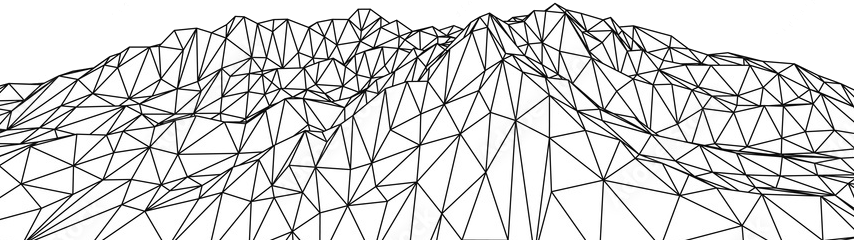
\includegraphics[width=\paperwidth]{../Unidad 2/Images/cover_bg}
\end{document}

\restoregeometry
\addtocontents{toc}{\setcounter{tocdepth}{3}}
\tableofcontents
\newpage
\chapter{}
\pagestyle{fancy}
\newpage \thispagestyle{plain}
\section{Múltiplos y divisores}
\subsection{Múltiplos}
\subsection{Divisores}
\subsection{Problemas de multiplicación y división de fracciones}
\subsection{Multiplicación de números positivos y negativos}

\newpage \thispagestyle{plain}
\section{Números primos}
\subsection{Números primos y compuestos}
\subsection{Factorización y descomposición en números primos}

\newpage \thispagestyle{plain}
\section{Mínimo común múltiplo y máximo común divisor}
\subsection{Mínimo común múltiplo}
\subsection{Máximo común divisor}

\newpage \thispagestyle{plain}
\section{Polígonos semejantes}
\subsection{Semejanza de polígonos}
\subsection{Construcción de polígonos semejantes}

\newpage \thispagestyle{plain}
\section{Criterios de semejanza de triángulos}
\subsection{Criterios de semejanza de triángulos}
\subsection{Aplicaciones de semejanza de triángulos}

\newpage \thispagestyle{plain}
\section{Medidas de tendencia central y de dispersión}
\subsection{Significado de las medidas de tendencia central}
\subsection{Significado de las medidas de dispersión}
\subsection{Comparación de dos conjuntos de datos}

\newpage
\chapter{}

\newpage \thispagestyle{plain}
\section{Ecuaciones cuadráticas}
\boxabstract{Analiza y compara diversos tipos de variación a partir de sus
  representaciones tabular, gráfi ca y algebraica, que resultan
  de modelar situaciones y fenómenos de la física y de otros
  contextos.}
\subsection{Ecuaciones cuadráticas}

Analiza las situaciones y contesta lo que se pide.\\

\begin{boxK}
  \begin{center}\textbf{Inicio}\end{center}
  Lee la situación, observa la imagen y responde lo que se pide.
  \begin{enumerate}
    \item Martín fue contratado para cercar un terreno con 120 m de malla. Le pidió a su cliente
          los datos del terreno, quien se los entregó en un papel. Al llegar a su casa, Martín se dio
          cuenta de que perdió la información y sólo recordó que el triple del ancho menos el
          largo es igual a 28 m. No quiso llamar nuevamente al cliente y determinó las dimensio-
          nes del terreno. \textbf{¿Cuáles son?}
          \begin{enumerate}
            \item Asigna variables y escribe las ecuaciones que modelan la situación.
            \item Describe un procedimiento para resolverlas.
            \item Determina las medidas de los lados del terreno.
            \item ¿Qué información es relevante para responder y
                  cuál no?
            \item Describe tu procedimiento para saber las respuestas.
          \end{enumerate}
  \end{enumerate}

\end{boxK}

\begin{enumerate}
  \item El hotel \emph{El Sol} gestionó con el municipio tener una zona de nado en el mar
        para el disfrute de sus huéspedes. Le han asignado 600 m$^2$ de superficie
        de mar y debe delimitarla con una cuerda y boyas para seguridad de los
        bañistas. El gerente del hotel quiere que la zona sea cuadrada, \\
        \textbf{¿cuál es la longitud de los lados? (figura \ref{fig:square})}.

        \begin{minipage}{.45\textwidth}
          \begin{figure}[H]
            \centering
            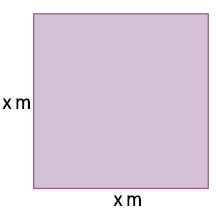
\includegraphics[width=0.7\linewidth]{square.png}
            \captionof{figure}{Modelo geométrico de la situación.}
            \label{fig:square}
          \end{figure}%
        \end{minipage}\hfill
        \begin{minipage}{.45\textwidth}
          \begin{figure}[H]
            \centering
            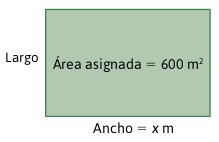
\includegraphics[width=0.8\linewidth]{square2.png}
            \captionof{figure}{Modelo geométrico de la situación.}
            \label{fig:square2}
          \end{figure}
        \end{minipage}

        \begin{enumerate}
          \item ¿Cuáles son las cantidades conocidas?
          \item ¿Cuáles son las cantidades desconocidas?
          \item Escriban una ecuación que modele la situación.
          \item ¿Cuál es la longitud de los lados?
        \end{enumerate}

  \item Antes de que se hiciera la delimitación de la zona de nado, el gerente del
        hotel cambió de opinión acerca de la forma de esta zona. Ahora debía
        ser rectangular con cierta característica: el largo tiene 10 m menos que
        el ancho. \textbf{¿Cuál es la longitud de los lados de la superficie delimitada?
          (figura \ref{fig:square2})}.\\
        \begin{enumerate}
          \item ¿Cuáles son las cantidades conocidas?
          \item ¿Cuáles son las cantidades desconocidas?
          \item Escriban una ecuación que modele la situación.
          \item Planteen una forma de resolver el problema. ¿Cuál es la longitud de los
                lados?
        \end{enumerate}

        \begin{boxH}
          Una \textbf{ecuación cuadrática} completa en una variable es una ecuación del tipo
          \begin{equation}
            ax^2 + bx + c = 0
          \end{equation}
          donde $a$, $b$ y $c$ son enteros, decimales o fraccionarios y $a$ no es igual a 0. Como el
          mayor exponente de la variable es 2 también se
          le conoce como \textbf{ecuación de segundo grado}.
        \end{boxH}

  \item Considera el problema anterior. El municipio ha
        notificado al gerente del hotel El Sol que hubo un error en la asignación de la zona
        de mar y que en lugar de 600 m$^2$ , se le asignan 504 m$^2$ . El gerente del hotel aún
        quiere que la zona de nado tenga 10 m menos de largo que de ancho. \textbf{¿Cuál es la
          nueva longitud de los lados?}

        \begin{enumerate}
          \item Identifiquen las cantidades conocidas, desconocidas y escriban una ecuación que
                modele la situación.
          \item Verifiquen cuáles valores son soluciones o raíces de la ecuación anterior y escriban
                por qué.
                \begin{itemize}
                  \item $x = -28$.
                  \item $x = -18$.
                  \item $x = -8$.
                  \item $x = 0$.
                  \item $x = 8$.
                  \item $x = 18$.
                  \item $x = 28$.
                \end{itemize}

        \end{enumerate}
\end{enumerate}
\begin{boxH}
  Un número que satisface una ecuación, es decir, que al sustituirlo en la variable de
  la ecuación se cumple la igualdad es llamado solución o raíz de la ecuación.
\end{boxH}

Completen la tabla \ref{tab:table01} sustituyendo los valores de x en cada expresión y haciendo las operaciones, luego respondan lo que se pide.

\begin{figure}[H]
  \centering
  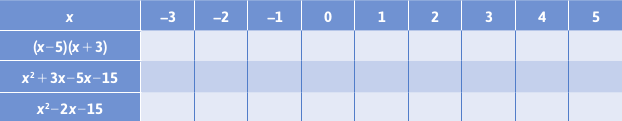
\includegraphics[width=0.5\textwidth]{tabla01.png}
  \captionof{figure}{Modelo geométrico de la situación.}
  \label{tab:table01}
\end{figure}

\begin{enumerate}
  \item ¿Cómo son los valores de las tres expresiones? ¿Qué pueden concluir sobre ellas?
  \item ¿Cómo pueden saber que un producto de expresiones algebraicas es equivalente a una ecuación de segundo grado?
\end{enumerate}


Se tienen dos expresiones algebraicas: $(x - 1)(x - 6) = 0$ y $x^2 - 7x + 6 = 0$.

\begin{enumerate}
  \item ¿Cuál es una ecuación cuadrática? ¿Por qué?
  \item ¿Cuántas soluciones tiene la ecuación (x - 1)(x - 6) = 0? Explica.
  \item ¿Cuántas soluciones tendrá la ecuación x$^2 - 7x + 6 = 0$? ¿Por qué?
  \item ¿Cuántas soluciones tendrá una ecuación cuadrática?
\end{enumerate}

Analicen los siguientes casos:
\[(x)(x) = 1 \text{\quad y \quad} x^2 = 1\]
\[x(x - 1) = 0 \text{\quad y \quad}x^2 - x = 0\]
\[(x - 1)(x - 2) = 0 \text{\quad y \quad} x^2 - 3x + 2 = 0\]
\[(x - 1)(x - 2) + 1 = 0 \text{\quad y \quad} x^2 - 3x + 3 = 0\]
Comprueben primero que
cada par de ecuaciones es equivalente. Pueden probar por ensayo y error para
encontrar las soluciones.\\

\begin{boxK}
  \begin{center}\textbf{Cierre}\end{center}
  \begin{enumerate}
    \item Retoma la situación de la actividad de inicio y responde, completa o corrige
          tus respuestas. ¿Qué pasaría con las soluciones de la ecuación si los 120 son
          metros cuadrados?
          Reflexiona acerca de los conocimientos o las habilidades que necesitabas al
          inicio y que ahora has adquirido. Escribe en tu cuaderno una conclusión.
    \item Los desarrolladores de un fraccionamiento habían planeado que algunos
          terrenos para construir las casas fueran de 20 por 40 metros, pero los
          40 m
          reducirán de tal manera que tengan 525 m$^2$ de área para ampliar los adadores, como se muestra en el bosquejo.
          \begin{enumerate}
            \item ¿De cuánto será el ancho del camino?
            \item ¿Cómo planteas la ecuación que permite resolver el problema?
          \end{enumerate}
  \end{enumerate}
\end{boxK}

\newpage
\subsection{Gr\'aficas de expresiones cuadráticas y soluciones de sus ecuaciones}
\begin{boxK}
  \begin{center}\textbf{Inicio}\end{center}
  \begin{enumerate}
    \item Lee la situación, observa la imagen y responde lo que se pide.
          La torre Eiffel tiene una altura de 324 m. Desde la parte superior se deja caer una pelota
          de golf. La gráfica que se muestra es la representación de la ecuación que describe este
          movimiento, sin considerar la resistencia del aire. \\
          \textbf{¿Cuánto tiempo tarda el objeto en llegar al suelo?}
          \begin{enumerate}
            \item ¿Qué parte de la gráfica tiene sentido considerar?
            \item ¿Qué altura corresponde al tiempo 0 s? ¿A qué tiempo corresponde la altura 0 m?
            \item ¿Qué valor es la solución del problema? Explica.
            \item ¿Qué significa en la situación el valor simétrico, es decir, de signo contrario, al que obtuviste en la pregunta anterior?
            \item ¿Qué información es relevante para responder y cuál no?
            \item Describe el procedimiento que realizaste para saber las respuestas.
          \end{enumerate}
    \item  Reúnanse en equipo. Comparen sus respuestas, argumenten. Corrijan si es necesario.
          Reflexionen sobre el uso de gráficas para describir y resolver ecuaciones.
          \begin{figure}[H]
            \centering
            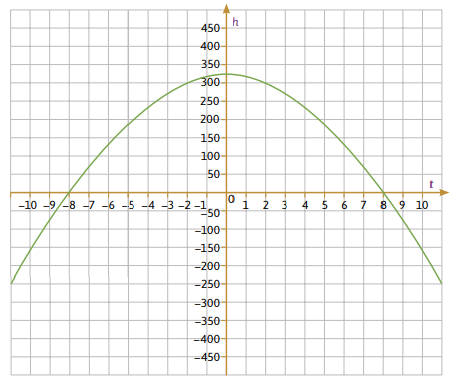
\includegraphics[width=0.65\textwidth]{parabole01.png}
            \captionof{figure}{Modelo geométrico de la situación.}
            \label{fig:parabole01}
          \end{figure}

  \end{enumerate}
\end{boxK}

\subsubsection{Soluciones de ecuaciones cuadráticas con gráficas}
Analizaremos diversas gráficas de variaciones cuadráticas para determinar
la relación entre éstas y las soluciones de la ecuación asociada.
2. Reúnanse en parejas. Hagan lo que se pide.
a) Analicen la gráfica de y = x2
(figura 2.3).
• Localicen los puntos en los que la gráfica interseca al eje X. ¿Cuál
es el valor de x en esos puntos?
• Sustituyan esos valores en la ecuación x2
= 0. ¿Qué observan?
• Elijan otros dos puntos que estén sobre la gráfica. ¿Cuál es el valor
de x en esos puntos?
• Sustituyan esos nuevos valores en la ecuación x2
= 0. ¿Qué observan?





\newpage \thispagestyle{plain}
\section{Resolución de ecuaciones cuadráticas}
\subsection{Procedimientos para la resolución de ecuaciones cuadráticas}
\subsection{Fórmula general de la ecuación de segundo grado}

\newpage \thispagestyle{plain}
\section{Relación entre variación y ecuación cuadrática}
\subsection{Variación cuadrática y ecuación asociada}
\subsection{Modelación de situaciones de variación cuadrática}

\newpage \thispagestyle{plain}
\section{Características de la variación}
\subsection{Distintos tipos de variación}
\subsection{Dependencia y razón de cambio}

\newpage \thispagestyle{plain}
\section{Análisis de la variación cuadrática}
\subsection{Representación tabular de la variación cuadrática}
\subsection{Representación algebraica de la variación cuadrática}
\subsection{Representación gr\'afica de la variación cuadrática}
\subsection{Representación tabular, algebraica y gr\'afica de variaciones cuadráticas}

\newpage \thispagestyle{plain}
\section{Variaciones diversas}
\subsection{Interpretación de gr\'aficas}
\subsection{Construcción de gr\'aficas a partir de tablas}
\subsection{Análisis de gr\'aficas de variaciones diversas}

\newpage \thispagestyle{plain}
\section{Eventos mutuamente excluyentes}
\subsection{Eventos singulares y no singulares}
\subsection{Eventos mutuamente excluyentes}
\subsection{Unión de dos eventos}
\subsection{Regla de la suma de probabilidades}

%%% U3
\chapter{}

\newpage \thispagestyle{plain}
\section{Expresiones algebraicas de segundo grado}
\subsection{Áreas y expresiones de segundo grado}
\subsection{Operaciones algebraicas}
\subsection{Factorización de expresiones de segundo grado}

\newpage \thispagestyle{plain}
\section{Expresiones algebraicas de ecuaciones y funciones}
\subsection{Expresiones algebraicas de ecuaciones}
\subsection{Expresiones algebraicas de funciones}

\newpage \thispagestyle{plain}
\section{Teorema de Pitágoras}
\subsection{Triángulos rectángulos y el teorema de Pitágoras}
\subsection{El teorema de Pitágoras}
\subsection{Aplicaciones del teorema de Pitágoras}

\newpage \thispagestyle{plain}
\section{Razones trigonométricas (seno, coseno y tangente)}
\subsection{Razones trigonométricas básicas}
\subsection{Razones trigonométricas de 30$^{\circ}$, 45$^{\circ}$ y 60$^{\circ}$}

\newpage \thispagestyle{plain}
\section{Resolución de triángulos rectángulos}
\subsection{Seno, coseno y tangente de ángulos agudos}
\subsection{Aplicaciones de razones trigonométricas}





\end{document}






